\scanpage{166}
\mspage{21}
qui devrait être contenue dans le formalisme, savoir (si $\unsure{k|h}$ alg clos disons) : \unsure{di|de|si} $F$ schéma abélien sur $K$, $F'$ le schéma abélien dual, et $G'$ le groupe proalgébrique sur $k$ attaché ``à la Greenberg'' à son modèle de Néron, on a
\[
 H^1(K,F)\overset{?}{\simeq}\operatorname{Ext}^{1}_{k\text{-}\unsure{\mathrm{gr}|\mathrm{gr.}|\mathrm{grp}}}(G',\unsure{Q|\mathbb Q}/\mathbb Z)
\]
(NB sans aucune garantie). En principe, la
% margin note written sideways
{\reversemarginpar\margin{\unsure{conj|conj.} \unsure{mentionnée} sur les modèles de Néron devrait sortir de la machine de dualité locale\par\noindent\tikz{\draw (0,.15) .. controls (.20,.15) and (.28,.10) .. (.32,-.04) .. controls (.32,.09) and (.43,.12) .. (.91,.12);}}}

d) Tu pourrais demander à Deligne s'il n'a pas approfondi les questions (D) et (E) dernièrement.

\figure{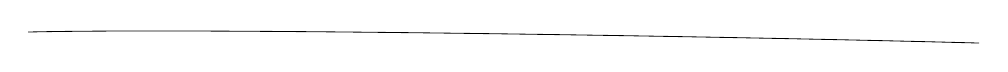
\begin{tikzpicture}[x=\linewidth,y=1cm]
\draw[line width=.3pt] (0,0) .. controls (.18,.05) and (.72,-.05) .. (.996,-.14);
\end{tikzpicture}}

(F) \uline{Portée et limites de la topologie} fppf

Depuis les essais de Serre de trouver une ``coh. de Weil'' en utilisant la cohomologie d'un schéma à coefficients non seulement discrets $\mathbb Z/p^n\mathbb Z$ ($n\unsure{\mapstochar\relbar\joinrel\dashv|\longrightarrow}\infty$), ou $\mu_{p^n}$ ($n\mathrel{\mapstochar\relbar\joinrel\dashv}\infty$), mais aussi continus (\inserted{p.ex} $W_n$, $n\unsure{\relbar\joinrel\dashv|\longrightarrow}\infty$), qui donnait de bons résultats pour récupérer un $H^1$ correct, pendant de nombreuses années j'étais \inserted{resté} sur l'impression, que j'essayais en vain de préciser, qu'une ``coh. de Weil'' ``$p$-adique''\unsure{:} correcte, en car. $p>0$, devait pouvoir sortir d'une façon ou d'une autre de la cohomologie fppf, pour des coefficients finis p.ex., ou des coefficients
% archive sheet number: 166
